\documentclass{article}
\usepackage{graphicx}
\usepackage[margin=1.5cm]{geometry}
\usepackage{amsmath}

\begin{document}

\title{Tuesday Reading Assessment: Chapters 6-1 through 6-6}
\author{Prof. Jordan C. Hanson}

\maketitle

\begin{figure}[ht]
\centering
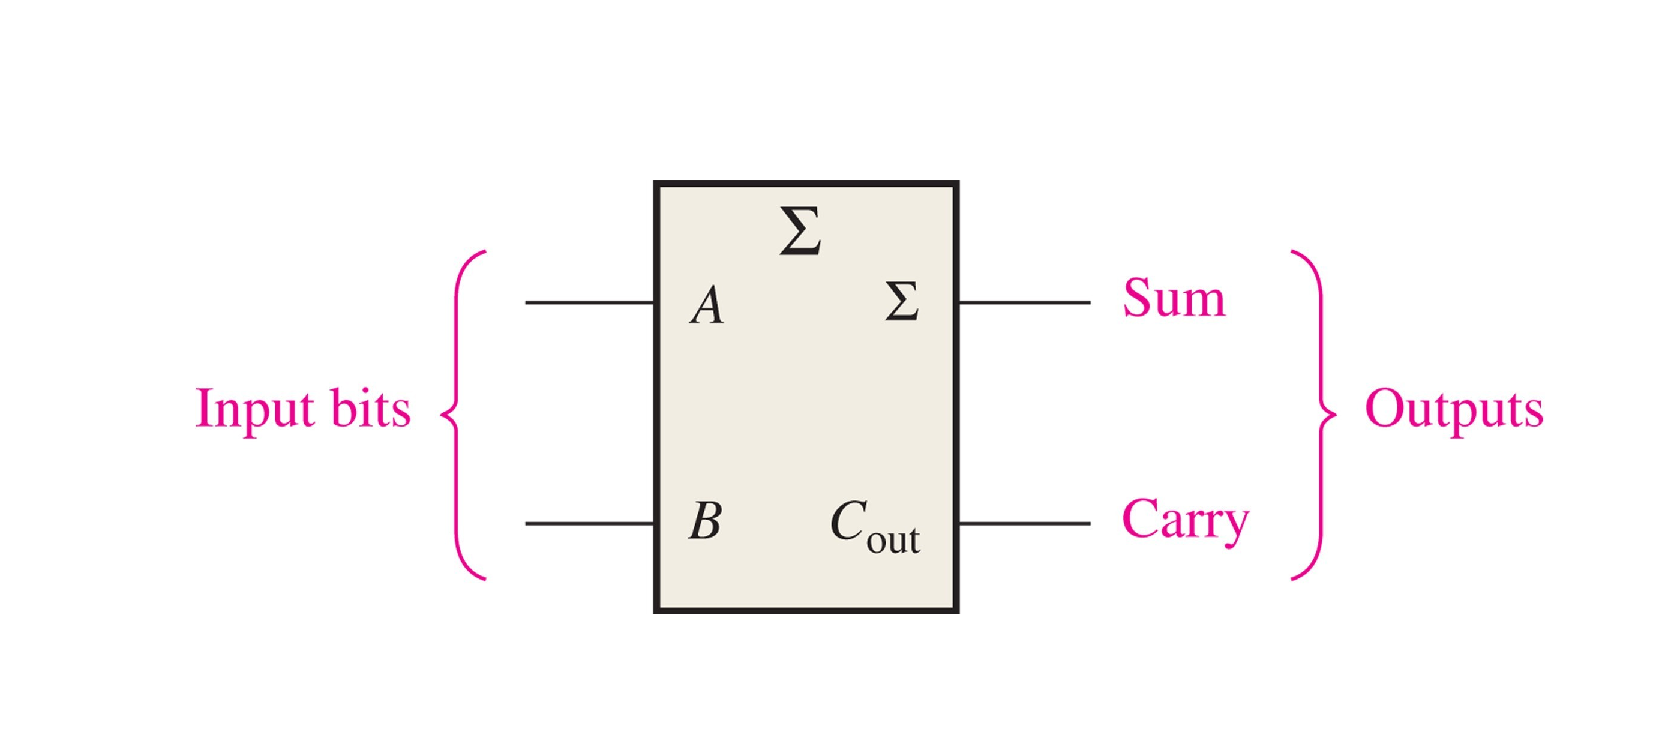
\includegraphics[width=0.45\textwidth]{figures/adder1.pdf} \hspace{0.5cm}
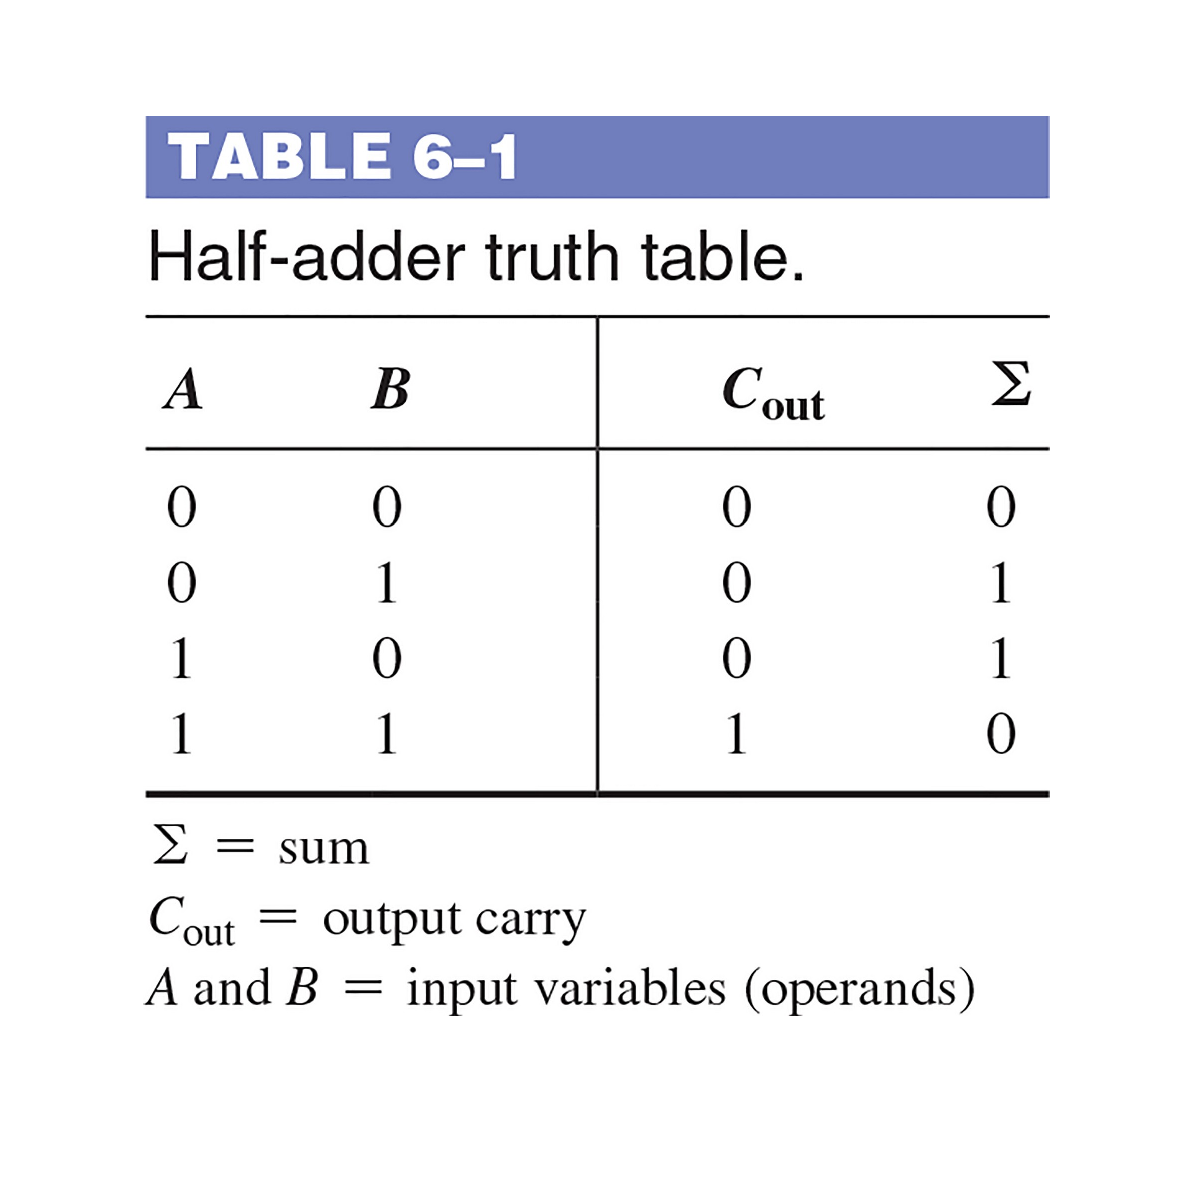
\includegraphics[width=0.25\textwidth]{figures/adder2.pdf}
\caption{\label{fig:1} (Left) Symbol for a \textit{half-adder}, that adds two bits and produces the sum and carry bits. (Right) The truth table for the sum and carry bits in terms of the input bits A and B.}
\end{figure}

\section{Functions of Combinatorial Logic: Adders}

\begin{enumerate}
\item Examine the $\Sigma$ (sum) output in the truth table in Fig. \ref{fig:1} (right).  What gate accurately describes $\Sigma$ in terms of the inputs A and B? \\ \vspace{0.5cm}
\item Examine the $C_{\rm out}$ (carry) output in the truth table in Fig. \ref{fig:1} (right).  What gate accurately describes $C_{\rm out}$ in terms of the inputs A and B? \\ \vspace{0.5cm}
\item Create a logic circuit schematic in the space below that functions like the component in Fig. \ref{fig:1} (left), producing the truth table in Fig. \ref{fig:1} (right). \\ \vspace{2.0cm}
\end{enumerate}

\section{Functions of Combinatorial Logic: Comparators}

\begin{enumerate}
\item (a) Write down the truth table for an XOR gate, but inverted (XNOR). (b) Use this truth table to create a circuit that is HIGH if two 2-bit binary numbers are equal.
\end{enumerate}

\end{document}
